\documentclass[tikz,border=2pt,11pt]{standalone}
\usetikzlibrary{calc}
\usetikzlibrary{arrows.meta}
\usetikzlibrary{patterns}
\usetikzlibrary{positioning}
\usepackage{amsmath}
\usepackage{amssymb}
\usepackage{tikz}
\newcommand{\T}{\mathbb T}
\newcommand{\Z}{\mathbb Z}
\newcommand{\R}{\mathbb R}
\newcommand{\N}{\mathbb N}
\newcommand{\A}{\mathbb A}
\newcommand{\PP}{\mathbb P}
\DeclareMathOperator{\Span}{span}
\DeclareMathOperator{\ord}{ord}
\DeclareMathOperator{\vol}{vol}
\DeclareMathOperator{\mult}{mult}
\DeclareMathOperator{\conv}{conv}
\DeclareMathOperator{\length}{length}
\DeclareMathOperator{\Spec}{Spec}
\DeclareMathOperator{\Proj}{Proj}
\DeclareMathOperator{\GL}{GL}
\begin{document}
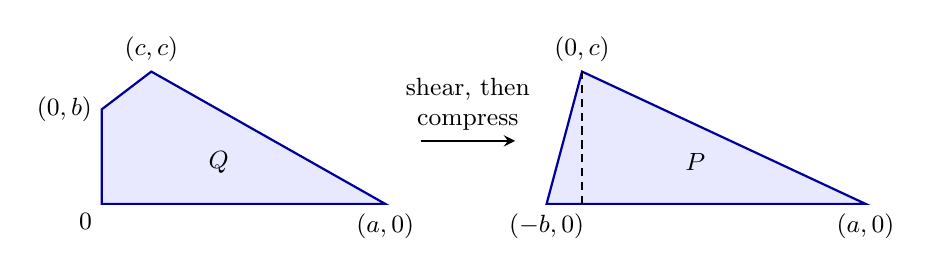
\begin{tikzpicture}[font=\small,>=stealth]
 \begin{scope}[xscale=.9,yscale=2.4]
  \filldraw[fill=blue!9,draw=blue!60!black,thick]
   (0,0)--(4,0)--(.7,.7)--(0,.5)--cycle;
  \node[below left] at (0,0) {$0$};
  \node[below] at (4,0) {$(a,0)$};
  \node[above] at (.7,.7) {$(c,c)$};
  \node[left] at (0,.5) {$(0,b)$};
  \node at (1.65,.22) {$Q$};
 \end{scope}
 \draw[->,thick] (4.05,.8)--(5.25,.8)
  node[midway,above,align=center] {shear, then\\compress};
 \begin{scope}[shift={(6.1,0)},xscale=.9,yscale=2.4]
  \filldraw[fill=blue!9,draw=blue!60!black,thick]
   (-.5,0)--(4,0)--(0,.7)--cycle;
  \draw[densely dashed] (0,0)--(0,.7);
  \node[below] at (-.5,0) {$(-b,0)$};
  \node[below] at (4,0) {$(a,0)$};
  \node[above] at (0,.7) {$(0,c)$};
  \node at (1.6,.22) {$P$};
 \end{scope}
\end{tikzpicture}
\end{document}
